\chapter{Fundamental Blocks of the Research} \label{chapter_two}


\section{Image Stabilisation}
What is image stabilisation?

% Start: Image Stabilisation
\subsection{Types of Image Stabilisation}
\subsubsection{Hardware Image Stabilisation}
Compensate camera movements with hardware. Expensive.

\subsubsection{Digital Image Stabilisation}
Compensate movements in post-processing. Economical.

\subsection{How Digital Image Stabilisation works}
We are interested in DIS so we will introduce the fundamentals.

% Start: IMU Sensors
\section{Inertial Measurement Unit Sensors}
An Inertial Measurement Unit (IMU) sensor measures acceleration(m/s²) and angular velocity (rad/s).  They can make these measurements in multiple degrees of freedom. For example, a 6-DoF IMU sensor includes a 3-axis accelerometer and 3 axis gyroscope  \citet{constant2021data}. The accelerometer will make independent acceleration measurements in let's say x, y and z directions. Similarly the gyroscope makes independent angular velocity measurements about these three axis.

IMU sensors are used in a wide variety of applications like navigation, robotics, drones, smart watches, sports learning, augmented reality systems, industrial quality control\citet{ahmad2013reviews}  and also for image stabilization in cameras. In all these applications, IMU sensor is used for pose estimation in some form. Either for absolute pose estimation or change in pose. It is important to note that for my application here the IMU will be strapped on to the camera system. Which means the IMU sensor can has all 6 of its DoF.

There are a lot of reasons to use IMU sensors and these reasons are surely a very huge contributor to them being on of the most commonly used sensors in the world. They have small size, low weight, rugged construction, low power consumption, cheap, high reliability, low maintenance and be used in hostile environments \citep{woodman2007introduction}.

\begin{itemize}
\item What are IMU Sensors?
\item What do they measure?
\item Applications?
\item Why use them for our application?
\item Advantages and Drawbacks
\end{itemize}

\subsection{Pose Estimation with IMUs}
Pose for any object is its position(x, y, z) and its orientation(yaw, pitch, roll) with respect to some reference coordinate system. To calculate pose of an object, we continuously take measurements from IMU and using some algorithms we calculate the pose. Figure \ref{fig:strapdown_imu} below shows the strap-down inertial navigation algorithm \citep{woodman2007introduction}.

\begin{figure}
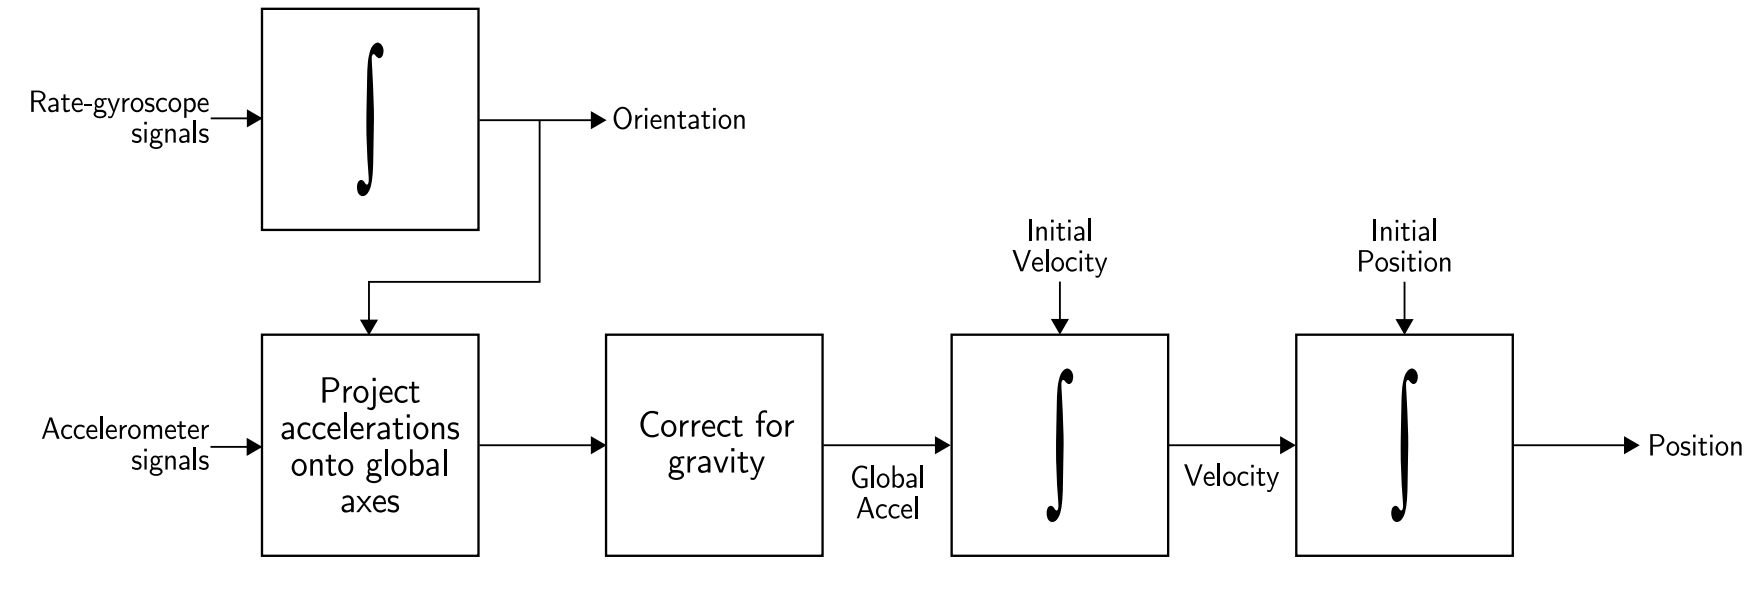
\includegraphics[scale=0.22]{images/fig_chapter1/strap_imu_algo.png}
\caption{Strap-down inertial navigation algorithm}
\label{fig:strapdown_imu}
\end{figure}

Based on the algorithm we can see that to estimate the pose, we need to do integration on Gyroscope values to get orientation. And double integration on Accelerometer values to get the position. That seems simple but the IMU readings are not ideal, they contain noises and biases \citep{woodman2007introduction} which need to be accounted for.

\subsection{Noise Models}
Sensors readings are inherent to noise. There is all kinds of noise which we have to deal with.


\subsubsection{Gyro Error Characteristics}
In table \ref{tab:gyro_error} you can see all errors in MEMS gyroscope.
% gyro error table
\begin{table}[ht]
    \centering
\begin{tabular}{ |l| L| L| } \hline
     \thead{Error Type} & \thead{Description} & \thead{Result of Integration} \\ \hline
     Bias & 
     A constant Bias epsilon & 
     Steadily growing angular error.theta(t) = epsilon*t  \\
     \hline
     White Noise & 
     White noise with some standard deviation sigma & 
     An angular random walk, whose standard deviation grows with the square root of time. \\
     \hline
     Temperature Effects & 
     Temperature dependent residual bias & 
     Any residual bias is integrated into orientation, causing an orientation error which grows linearly with time. \\
     \hline
     Calibration & 
     Deterministic errors in scale factors, alignments and gyro linearities & 
     Orientation drift proportional to the rate and duration of motion. \\
     \hline
     Bias Instability & 
     Bias fluctuations, usually modelled as a bias random walk & 
     A second order random walk. \\
     \hline
\end{tabular}
    \caption{Summary of Gyro Error Sources \citep{woodman2007introduction}}
    \label{tab:gyro_error}
\end{table}

\subsubsection{Accelerometer Error Characteristics}
In table \ref{tab:accel_error} you can see all errors in an MEMS accelerometer.
% accelerometer error table
\begin{table}[ht]
    \centering
\begin{tabular}{ |l| L| L| } \hline
     \thead{Error Type} & \thead{Description} & \thead{Result of Double Integration} \\ \hline
     Bias & 
     A constant Bias epsilon in the accelerometer's output signal. & 
     A quadratically growing position error. s(t) = epsilon * (t²)/2  \\
     \hline
     White Noise & 
     White noise with some standard deviation sigma & 
     A second order random walk. The standard deviation of the position error grows as sigmas(t) = sigma.. \\
     \hline
     Temperature Effects & 
     Temperature dependent residual bias & 
     Any residual bias causes an error in position which grows quadratically with time. \\
     \hline
     Calibration & 
     Deterministic errors in scale factors, alignments and accelerometer linearities & 
     Position drift proportional to the squared rate and duration of acceleration. \\
     \hline
     Bias Instability & 
     Bias fluctuations, usually modelled as a bias random walk & 
     A third-order random walk in position. \\
     \hline
\end{tabular}
    \caption{Summary of Accelerometer Error Sources \citep{woodman2007introduction}}
    \label{tab:accel_error}
\end{table}

\subsection{Challenges in Working with IMU}
As you can see it is not straightforward to work with IMUs, especially for absolute position estimation as the errors introduced are squared with time. This presents a lot of challenges especially for our case, as we require a precision in the range 1/10 of a mm. So, the sensor readings cannot be used directly in the inertial navigation algorithm. Generally some advanced signal processing techniques and algorithms (Kalman Filter, Extended Kalman Filter, 6 DoF Kalman Filter) are used to estimate the pose using IMU. These techniques may be good enough for some other applications, but in our case their use is not enough. The precision requirements are very high. Even if we use these algorithms, there is still a drift present which is unacceptable for this use case.

% Start: Neural Networks
\section{Neural Network Architectures Explained}
We will be using a lot of Neural Networks. The basic functioning of them is explained here.

\subsection{Multi Layer Perceptron}
Most basic ANN.

\subsection{Convolutional Neural Networks}
More advanced neural networks.

\subsection{Recurrent Neural Networks}
Neural networks with memory.

\subsection{Attention Mechanism}
Talk about attention in Neural Networks.

\subsection{Transformer Networks}
How self attention is used in Neural Networks.
